 \appendtographicspath{
          {python_submodule/figures/}
          {pytorch_submodule/src/the_framework/graph_acquisition/figures/}
          {pytorch_submodule/src/the_framework/graph_acquisition/figures/}
          }


\section{Pytorch Basics\hfill\normalsize{\pythoninline{import torch.tensor}}}
  \section*{PyTorch Folder Sturcutre}
    \begin{sectionbox}\nospacing
\dirtree{%
    .1 / (Project Root).
    .2 c10/ \DTcomment{C10 Library}.
    .3 src/ \DTcomment{C10 source code}.
    .2 aten/ \DTcomment{ATen Library}.
    .3 src/ \DTcomment{ATen source code}.
    .2 torch/ \DTcomment{Python Tensor Library}.
    .3 \_tensor.py .
    .3 autograd/ \DTcomment{Python Autograd Interface}.
    .3 \ldots \DTcomment{All the other Python components}.
    .3 csrc/ \DTcomment{C++ Core based on C10/ATen}.
    .4 autograd/ \DTcomment{C++ Autograd Infrastructure}.
    .4 interfaces/ \DTcomment{Interfaces to ATen and C10}.
    .4 \ldots \DTcomment{All other C++ implementations}.
}
\end{sectionbox}
%%% Local Variables:
%%% mode: latex
%%% TeX-command-extra-options: "-shell-escape"
%%% TeX-master: "../../../../../formulary"
%%% End:


  \section*{Torch}
    \subsection{Tensors}
      \begin{defnbox}\nospacing
    \begin{defn}[Tensor]\label{defn:tensor}\leavevmode\\
        Is the fundamental data structure for efficient computations in Pytorch:
        \begin{mintlinebox}{python}
            x = tensor(|\texttt{\optc{data}}|, |\texttt{\optc{[}device=\optc{device]}}|)
        \end{mintlinebox}
    \end{defn}
\end{defnbox}
\begin{corbox}\nospacing
    \begin{cor}[Implementation Details]\label{cor:torch_tensor_implementation_details}\leavevmode\\
        \pythoninline{torch.tensors} are based on the C++ ATen\cref{defn:aten} class \cppinline{at::Tensor} see \cref{defn:at::Tensor}.
    \end{cor}
\end{corbox}
%%% Local Variables:
%%% TeX-command-extra-options: "-shell-escape"
%%% mode: latex
%%% TeX-master: "../../../../../formulary"
%%% End:

      \subsubsubsection*{Important Tensor Attributes}\label{subsubsubsec:tensor_methods}
        \input{pytorch_submodule/src/the_framework/basics/tensors/attributes.tex}
        \paragraph{Shape and Size}
          % tensor.shape: Returns the dimensions (shape) of the tensor.
          % tensor.size(): Returns the size of the tensor (total number of elements).
        \paragraph{Data Type and Device}
          % tensor.dtype: Returns the data type of the elements in the tensor.
          % tensor.device: Returns the device (CPU or CUDA) on which the tensor is located.
      \subsubsubsection*{Important Tensor Methods}\label{subsubsubsec:tensor_methods}
        \paragraph{Data Generation}
          \begin{methodbox}{\pythoninline{torch.zeros(|\texttt{\optc{shape}}|)}}\leavevmode
    zeros
\end{methodbox}
\begin{methodbox}{\pythoninline{torch.ones(|\texttt{\optc{shape}}|)}}\leavevmode
    ones
\end{methodbox}
\begin{methodbox}{\pythoninline{torch.rand(|\texttt{\optc{shape}}|)}}\leavevmode
    uniformily distributed data.
\end{methodbox}
\begin{methodbox}{\pythoninline{torch.randn(|\texttt{\optc{shape}}|)}}\leavevmode
    normally distributed data.
\end{methodbox}

%%% Local Variables:
%%% mode: latex
%%% TeX-command-extra-options: "-shell-escape"
%%% TeX-master: "../../../../../formulary"
%%% End:

          % torch.empty(): Generates a 1-D tensor with regularly spaced values within a specified range.
          % torch.arange(): Generates a 1-D tensor with regularly spaced values within a specified range.
          % torch.linspace(): Generates a 1-D tensor with a specified number of equally spaced values within a range.
        \paragraph{Combining Tensors}
          \begin{methodbox}{\pythoninline{torch.cat(ten1, ten2, |\texttt{\optal,dim=0\optar}|)}}\leavevmode\\
    concatenates two tensors along dim (rowise stacking by default).
\end{methodbox}
%%% Local Variables:
%%% mode: latex
%%% TeX-command-extra-options: "-shell-escape"
%%% TeX-master: "../../../../../formulary"
%%% End:

          % torch.stack(): Stacks a sequence of tensors along a new dimension.
        \paragraph{Transforming Tensors}
            % tensor.view(): Reshapes the tensor to a specified shape.
            % tensor.reshape(): Reshapes the tensor to a specified shape.
            % tensor.transpose(): Transposes the dimensions of the tensor.
            % tensor.permute(): Permutes the dimensions of the tensor according to the given order.
            % tensor.squeeze(): Removes dimensions with size 1.
            % tensor.unsqueeze(): Adds a dimension with size 1.
            % .t() / tensor.transpose() / .T: Transposes a Tensor
        \paragraph{Mathematical Operations}
            % torch.add() / +: Adds two tensors element-wise.
            % torch.sub() / -: Subtracts one tensor from another element-wise.
            % torch.mul() / *: Multiplies two tensors element-wise.
            % torch.div() / /: Divides one tensor by another element-wise.
            % torch.exp(): Computes the exponential of each element.
            % torch.log(): Computes the natural logarithm of each element.
            % torch.sqrt(): Computes the square root of each element.
            % torch.sum(): Computes the sum of elements along specified dimensions.
            % torch.mean(): Computes the mean of elements along specified dimensions.
            % torch.max(): Computes the maximum element along specified dimensions.
            % torch.min(): Computes the minimum element along specified dimensions.
        \paragraph{Matrix Operations}
            % torch.mm() / @: Performs matrix multiplication.
            % torch.bmm(): Performs batch matrix multiplication.
            % torch.matmul(): Performs matrix multiplication with broadcasting.
        \paragraph{Logical Comparisons}
            % torch.eq(): Element-wise equality comparison.
            % torch.gt(): Element-wise greater than comparison.
            % torch.lt(): Element-wise less than comparison.
            % torch.logical_and(): Element-wise logical AND operation.
        \paragraph{Misc}
          \begin{methodbox}{\pythoninline{to(|\texttt{\optc{device}}|)}}\leavevmode
    move tensor to device.
\end{methodbox}
%%% Local Variables:
%%% mode: latex
%%% TeX-command-extra-options: "-shell-escape"
%%% TeX-master: "../../../../../../formulary"
%%% End:

            % tensor.item(): Returns the value of a tensor as a standard Python number if the tensor contains a single element.
            % tensor.detach(): Returns the value of a tensor as a standard Python number if the tensor contains a single element.
        \paragraph{In-place operations \pythoninline{op_}}



\newpage
  \subsection{Tracing}
  \begin{defnbox}\nospacing
    \begin{defn}[Symbolic Tracing]\label{defn:symbolic_tracing}\leavevmode\\
        \begin{minipage}[c]{0.52\textwidth}
            Is the capture and representation of python operations as a symbolic graph.
        \end{minipage}\hfil
        \begin{minipage}{0.4\textwidth}
            \begin{figure}[H]
                \centering
                
\includegraphics[width=0.9\textwidth]{pytorch_submodule/src/the_framework/graph_acquisition/figures/code_to_graph.pdf}
            \end{figure}
        \end{minipage}
    \end{defn}
\end{defnbox}

\begin{defnbox}\nospacing
    \begin{defn}[Computation Graph]\label{defn:computation_graph}\leavevmode\\
        A computation graph is a representation that can tracks data flow and operations and that can be used for automatic differentiation.
    \end{defn}
\end{defnbox}
\begin{defnbox}\nospacing
    \begin{defn}[Dynamic Graph Computation]\label{defn:dynamic_graph_computation}\leavevmode\\
        A dynamic graph is a graph that tracks operations and data flow dynamically during the execution of the code.
    \end{defn}
\end{defnbox}


%%% Local Variables:
%%% mode: latex
%%% TeX-command-extra-options: "-shell-escape"
%%% TeX-master: "../../../../formulary"
%%% End:

  \subsection*{Automatic Differentiation}\label{subsec:automatic_differentiation}
    \begin{defnbox}\nospacing
    \begin{defn}[Automatic Differentiation]\label{defn:automatic_differentiation}

    \end{defn}
\end{defnbox}

%%% Local Variables:
%%% mode: latex
%%% TeX-command-extra-options: "-shell-escape"
%%% TeX-master: "../../../../../formulary"
%%% End:

    \subsubsection{Reverse Modoe AD}\label{subsubsec:reverse_modoe_ad}
      \begin{defnbox}\nospacing
    \begin{defn}[\newline Reverse Mode Automatic Differentiation]\label{defn:reverse_mode_automatic_differentiation}\leavevmode\\

    \end{defn}
\end{defnbox}

%%% Local Variables:
%%% mode: latex
%%% TeX-command-extra-options: "-shell-escape"
%%% TeX-master: "../../../../../formulary"
%%% End:



  \section*{Torch Eager Mode}\label{subsec:torch_eager_mode}
      \begin{defnbox}\nospacing
    \begin{defn}[Eager Mode]\label{defn:eager_mode}\leavevmode\\
        Eager mode is the default PyTorch mode, operations are executed immediately like in normal Python code.

        In order to do automatic differentiation (AD) for gradient calculation during the backward pass, eager mode needs to track the operations performed on tensors
        by building a dynamic graph\cref{defn:dynamic_graph_computation}.

        This graph can be traversed backwards to calculate the gradients for each operation.
    \end{defn}
\end{defnbox}
\begin{sectionbox}\nospacing
   \begin{proslist}
       \item \pythoninline{print} immediate results
       \item debug control flows (e.g. loops and conditionals) line by line
       \item fast prototyping
   \end{proslist}
   \begin{conslist}
       \item builds a dynamic graph on the fly, as operations are performed\\
        $\Rightarrow$ graph compilation and optimizations such as fusions of operations not possible
   \end{conslist}
\end{sectionbox}
\begin{defnbox}\nospacing
    \begin{defn}[Computation Graph]\label{defn:computation_graph}\leavevmode\\
        A computation graph is a representation that can tracks data flow and operations and that can be used for automatic differentiation.
    \end{defn}
\end{defnbox}
\begin{defnbox}\nospacing
    \begin{defn}[Dynamic Graph Computation]\label{defn:dynamic_graph_computation}\leavevmode\\
        A dynamic graph is a graph that tracks operations and data flow dynamically during the execution of the code.
    \end{defn}
\end{defnbox}

%%% Local Variables:
%%% mode: latex
%%% TeX-command-extra-options: "-shell-escape"
%%% TeX-master: "../../../../../formulary"
%%% End:

    \subsection*{Automatic Differentiation \rb{AD}}\label{subsec:automatic_differentiation}
      \begin{defnbox}\nospacing
    \begin{defn}[Automatic Differentiation]\label{defn:automatic_differentiation}

    \end{defn}
\end{defnbox}

%%% Local Variables:
%%% mode: latex
%%% TeX-command-extra-options: "-shell-escape"
%%% TeX-master: "../../../../../formulary"
%%% End:

      \subsubsubsection{Gradient Computation}\label{subsubsec:gradient_computation}
          \begin{defnbox}\nospacing
    \begin{defn}[Gradient Computation]\label{defn:gradient_computation}

    \end{defn}
\end{defnbox}

    \subsection*{Tensors, Graphs and AutoGrad}\label{subsubsec:autograd}\stepcounter{subsection}
        \begin{defnbox}\nospacing
    \begin{defn}[Tensor]\label{defn:tensor}\leavevmode\\
        Is the fundamental data structure for efficient computations in Pytorch:
        \begin{mintlinebox}{python}
            x = tensor(|\texttt{\optc{data}}|, |\texttt{\optc{[}device=\optc{device]}}|)
        \end{mintlinebox}
    \end{defn}
\end{defnbox}
\begin{corbox}\nospacing
    \begin{cor}[Implementation Details]\label{cor:torch_tensor_implementation_details}\leavevmode\\
        \pythoninline{torch.tensors} are based on the C++ ATen\cref{defn:aten} class \cppinline{at::Tensor} see \cref{defn:at::Tensor}.
    \end{cor}
\end{corbox}
%%% Local Variables:
%%% TeX-command-extra-options: "-shell-escape"
%%% mode: latex
%%% TeX-master: "../../../../../formulary"
%%% End:

        \subsubsection*{grad\_fn}\label{subsubsec:grad_fn}
          \begin{sectionbox}[Eager Mode Execution]\nospacing
    \begin{circlelistnosep}
        \item
    \imp{Operation Execution}:\\
    During eager-execution, a \pythoninline{grad_fn} is created for each operation.
    For each input tensor \pythoninline{collect_next_edges} adds an edge to the \pythoninline{grad_fn} of the input tensor and adds the link to \pythoninline{grad_fn.next_functions} array.\\
    For input tensors without a \pythoninline{grad_fn}, \pythoninline{collect_next_edges} links to the special function \pythoninline{AccumulateGrad}.
    \item \imp{Backward}:
    \pythoninline{Autograd} calcualtes the gradients using the rules of \pythoninline{grad_fn} and accumulates results into the \pythoninline{grad} fields of the tensors.
    \end{circlelistnosep}
    \begin{figure}[H]
        \centering
        
\includegraphics[width=1.0\textwidth]{pytorch_submodule/src/the_framework/basics/automatic_differentiation/autograd/figures/graph.pdf}
    \end{figure}
\end{sectionbox}
\begin{defnbox}\nospacing
    \begin{defn}[\tcblack{\pythoninline{grad_fn}}]\leavevmode\\
        Is the main function object that:
        \begin{itemizenosep}
            \item represents operations and their derivatives
            \item represents nodes in the computational graphs and links to the previous functions that created the current tensor using \pythoninline{grad_fn.next_functions}.
        \end{itemizenosep}
    \end{defn}
\end{defnbox}
\begin{defnbox}\nospacing
    \begin{defn}[\tcblack{\pythoninline{grad_fn.next_functions}}]\leavevmode\\
        Is an array of \pythoninline{grad_fn, pos} tuples, where
        \begin{itemizenosep}
            \item the \pythoninline{grad_fn} points to the previous (older for in-forward) operation
            \item \pythoninline{pos} represents the position of the current tensor in the \pythoninline{grad_fn} of the previous input tensor
        \end{itemizenosep}
    \end{defn}
\end{defnbox}
\begin{notebox}[Notes]\nospacing
    \begin{itemizenosep}
        \item Position is important for the backward pass and functions such as \pythoninline{unbind} which needs to know during automatic differention, which tensor is which: \pythoninline{b, c, a = a.unbind()}
        \item Non leaf gradients are not calculated as the can be calculated implicitly
    \end{itemizenosep}
\end{notebox}
%%% Local Variables:
%%% mode: latex
%%% TeX-command-extra-options: "-shell-escape"
%%% TeX-master: "../../../../../../formulary"
%%% End:

        \subsubsection*{AutoGrad\hfill\normalsize{\pythoninline{from torch import autograd}}}\label{subsubsec:name}
          \begin{defnbox}\nospacing
    \begin{defn}[Autograd]\label{defn:autograd}\leavevmode\\
        \pythoninline{torch.autograd} is Pytorchs automatic differentiation module.
    \end{defn}
\end{defnbox}
\begin{defnbox}\nospacing
    \begin{defn}[\pythoninline{autograd.grad}]\leavevmode\\
       Calculates the gradient of an input tensor $x$ w.r.t.\ an output tensor $y$:
        \begin{mintlinebox}{python}
            x = torch.tensor(3.0, requires_grad=True)
            y = x ** 2
            grad_y_x = autograd.grad(y, x)
        \end{mintlinebox}
    \end{defn}
\end{defnbox}
\begin{defnbox}\nospacing
    \begin{defn}[\pythoninline{autograd.backward}]\leavevmode\\
        calculates all the gradients of all the tensors that are marked for gradient computation (\pythoninline{requires_grad=True})
        w.r.t.\ to a graph of a given tensor $y$ and accumulates the respective gradients into the \pythoninline{grad} fields of the tensors:
        \begin{mintlinebox}{python}
            x = torch.tensor(3.0, requires_grad=True)
            y = x ** 2
            # populate: x.grad and y.grad
            y.backward()
        \end{mintlinebox}
    \end{defn}
\end{defnbox}
\begin{attentionbox}{Attention}\nospacing \leavevmode
    \begin{itemizenosep}
        \item As of now, \pythoninline{autograd} only supports floating point and complex Tensor types.
        \item We can call \pythoninline{grad}/\pythoninline{backward} only once, unless with set \pythoninline{retain_graph=True}
        \item \pythoninline{y.backward()} is actually an alias for:\\ \pythoninline{autograd.backward(y, torch.ones_like(y))} as $\pdv{y}{y}=\vec{1}$.
    \end{itemizenosep}
\end{attentionbox}
\paragraph{Options}\label{para:options}
\begin{optionsbox}\nospacing
    \begin{option}[\pythoninline{retain_graph=None}]
          specifies whether to discard the graph after automatic differentiation.
    \end{option}
\end{optionsbox}


%%% Local Variables:
%%% mode: latex
%%% TeX-command-extra-options: "-shell-escape"
%%% TeX-master: "../../../../../../formulary"
%%% End:

        \subsubsection*{The Dispatcher}\label{subsubsec:dispatch}


      \subsection*{Grad Modes}\label{subsubsubsec:grad_modes}\stepcounter{subsubsection}
      \subsubsection{Grad Mode}
      \subsubsection{No-Grad Mode\hfill\normalsize{\pythoninline{torch.no_grad}}}
        \begin{defnbox}\nospacing
    \begin{defn}[No Grad]\label{defn:no_grad}\leavevmode\\
        Is a thread local context manager\cref{defn:context_manager} that allows to disable gradient computation in its context:\\
        \imp{Using \pythoninline{with}}:
        \begin{mintlinebox}{python}
        x = torch.tensor(1.0, requires_grad=True)
        with torch.no_grad():
            |\texttt{\optc{some tensor operations with x}}|
        \end{mintlinebox}
        \imp{As decorator}:
        \begin{mintlinebox}{python}
        @torch.no_grad()
        def fu(|\texttt{\optc{args}}|):
            |\texttt{\optc{some tensor operations}}|
        \end{mintlinebox}
    \end{defn}
\end{defnbox}
\begin{notebox}[Note]\nospacing
    Output tensors inside this context will have \pythoninline{requires_grad=False}, even for input tensors with \pythoninline{requires_grad=True}.
\end{notebox}
%%% Local Variables:
%%% mode: latex
%%% TeX-command-extra-options: "-shell-escape"
%%% TeX-master: "../../../../../../../../formulary"
%%% End:

      \subsubsection{Inference Mode}
      \subsubsection{Evaluation Mode}
      % (disables dropout etc)
      \subsection*{Custom AutoGrad Operations}
        % \paragraph{Using The Python API\hfill\normalsize{\pythoninline{from torch.autograd import Function}}}
        % https://pytorch.org/tutorials/beginner/examples_autograd/two_layer_net_custom_function.html
        % https://pytorch.org/docs/stable/generated/torch.autograd.function.FunctionCtx.save_for_backward.html
      \subsection*{\tc{gray}{\textit{AutoGrad Profiler - Legacy}}}\label{subsubsubsec:grad_modes}


\section{PyTorch Internals--Graph Acquisition}
  \subsection*{Torch Compile}\label{subsec:torch_compile}\stepcounter{subsection}
    \begin{sectionbox}[Why do we need torch compile?]\nospacing
        Efficient computation graphs are important for modern deep learning applications.
        Dynamic graph computation\cref{defn:dynamic_graph_computation} for eager mode\cref{defn:eager_mode} frameworks used to work as fast as compiled graph frameworks.
        \begin{figure}[H]
            \centering
            \includegraphics[width=1.0\textwidth]{pytorch_submodule/src/the_framework/graph_acquisition/figures/overview.png}
        \end{figure}
        This used to be true as long as batch sizes are small and operations are simple.
        I.e. the execution of the \textit{host} python code (+graph acquisition) used to be faster than the execution of the kernels queuing on the GPU.
        However modern accelerators are getting faster, operations getting complexer and batch size are getting bigger such that graph acquisition on the host becomes the bottleneck.
\end{sectionbox}

%%% Local Variables:
%%% mode: latex
%%% TeX-command-extra-options: "-shell-escape"
%%% TeX-master: "../../../../formulary"
%%% End:

    \begin{defnbox}\nospacing
    \begin{defn}[Torch Compile]\label{defn:torch_compile}
        Torch compile is a JIT compiler that consists of:
        \begin{circlelistnosep}
            \item TorchDynamo\cref{defn:torch_dynamo}
            \item AOTAutograd\cref{defn:aotautograd}
            \item ATen IR\cref{defn:aten_a_tensor_library}
            \item TorchInductor\cref{defn:torchinductor}
        \end{circlelistnosep}
        it can be used for graph acquisition and optimization:
        \begin{mintlinebox}{python}
           import torch
           import torch._dynamo as dynamo
           cmp_f = torch.compile(
               |\texttt{\optc{(fun/module)}}|, backend=|\texttt{\optc{backend}}|
           )
        \end{mintlinebox}
    \end{defn}
\end{defnbox}
\begin{notebox}[Resetting The Backend]\nospacing
    Note, if we change the backend we need to first reset the dynamo default backend:
    \begin{plaincodebox}[colback=notebox]{python}
    dynamo.reset()
    \end{plaincodebox}
\end{notebox}


%%% Local Variables:
%%% mode: latex
%%% TeX-command-extra-options: "-shell-escape"
%%% TeX-master: "../../../../formulary"
%%% End:

    \subsection*{Torch FX}\label{subsec:fx_graph}
      \begin{defnbox}\nospacing
    \begin{defn}[Torch FX]\label{defn:torch_fx}\leavevmode\\
        Torch FX is a system that enables python-to-python code transformations of Pytorch code.
        Torch FX consists of three  main components:
        \begin{circlelistnosep}
            \item \textit{\tc{gray}{Symbolic Tracing - legacy}}:\\
            \tc{gray}{\texttt{torch.fx.trace} feeds \textit{proxies} (=fake values) through the code to record operations that can be represented as an FX IR.}\\
            \tc{gray}{(will be most likely discontinued for Dynamo\cref{defn:torch_dynamo})}
            \begin{mintlinebox}{python}
                from troch.fx import Tracer, Graph
                def fu(x):
                    return torch.relu(x).neg()
                graph : Graph = Tracer(fu)
            \end{mintlinebox}
            \item Torch FX Intermediate Representation (IR): \\
            \textit{Torch FX IR} is the container for the operations that are recorded during symbolic tracing\cref{defn:torch_fx_ir}.
            \begin{mintlinebox}{python}
                from troch.fx import symbolic_trace, GraphModule
                gm : GraphModule = torch.fx.symbolic_trace(fu)
            \end{mintlinebox}
            \item Python Code Generation:\\
            Is the Python-to-Python tool that takes an FX Graph IRs represented as \pythoninline{torch.fx.GraphModule} as input and creates a transformed Python output that respects the graph semantics.
            \begin{mintlinebox}{python}
                print(gm.code)
            \end{mintlinebox}
        \end{circlelistnosep}
    \end{defn}
\end{defnbox}
\begin{defnbox}\nospacing
    \begin{defn}[Torch FX IR\hfill\tcblack{\pythoninline{torch.fx.Graph}}]\label{defn:torch_fx_ir}\leavevmode\\
        Torch IR is represented by a DAG where, Nodes represent operations and edges represent values.
        \pythoninline{torch.fx.Graph} is the format and underlying structure on which  transformations can be applied:
        \begin{mintlinebox}{python}
           print(graph)
        \end{mintlinebox}
    \end{defn}
\end{defnbox}
\begin{defnbox}\nospacing
    \begin{defn}[\hfill\tcblack{\pythoninline{torch.fx.GraphModule}}\newline Torch FX Code Generation]\label{defn:torch_fx_code_generation}\leavevmode\\
        The \pythoninline{GraphModule} is generated from an \pythoninline{fx.Graph}.


        A \pythoninline{GraphModule} is an \pythoninline{nn.Module} that has
        \begin{itemizenosep}
            \item a \pythoninline{fx.Graph} attribute
            \item a \pythoninline{fx.code} attribute representing the generated code
            \item a \pythoninline{fx.forward} attribute generated from the corresponding graph
        \end{itemizenosep}
        \begin{mintlinebox}{python}
            def transform(m: nn.Module, tracer_class = torch.fx.Tracer)
                    -> torch.nn.Module:
              graph : torch.fx.Graph = tracer_class().trace(m)
              graph = |\texttt{\optc{modify(\tcblack{graph})}}|
              return torch.fx.GraphModule(m, graph)
        \end{mintlinebox}
    \end{defn}
\end{defnbox}


%%% Local Variables:
%%% mode: latex
%%% TeX-command-extra-options: "-shell-escape"
%%% TeX-master: "../../../../../formulary"
%%% End:

    \subsection{\tc{gray}{\textit{FX Tracing - Legacy}}}
    \subsection{Torch Dynamo\hfill\normalsize{\pythoninline{import torch._dynamo as dynamo}}}
      \begin{sectionbox}[Why Torch Dynamo?]\nospacing
    Why do we need Torch Dynamo if we have Torch Script \pythoninline{torch.jit} and
    Torch FX tracing \pythoninline{torch.fx.symbolic_trace}?\\

\end{sectionbox}
\begin{defnbox}\nospacing
    \begin{defn}[Torch Dynamo]\label{defn:torch_dynamo}\leavevmode\\
        Torch Dynamo is a JIT compiler that generates \textit{FX Graphs}\cref{defn:fx_graph} from Python bytecode.\\
        It uses the frame evaluation API in CPython to dynamically modify Python bytecode before execution.\\
        This modified python bytecode is then extracted into an FX Graph which can then be just-in-time compiled with a suitable backend.
        \begin{figure}[H]
            \vspace{-1em}
            \centering{
              \def\svgwidth{200pt}
              \resizebox{\linewidth}{!}{\begin{sectionbox}[Why Torch Dynamo?]\nospacing
    Why do we need Torch Dynamo if we have Torch Script \pythoninline{torch.jit} and
    Torch FX tracing \pythoninline{torch.fx.symbolic_trace}?\\

\end{sectionbox}
\begin{defnbox}\nospacing
    \begin{defn}[Torch Dynamo]\label{defn:torch_dynamo}\leavevmode\\
        Torch Dynamo is a JIT compiler that generates \textit{FX Graphs}\cref{defn:fx_graph} from Python bytecode.\\
        It uses the frame evaluation API in CPython to dynamically modify Python bytecode before execution.\\
        This modified python bytecode is then extracted into an FX Graph which can then be just-in-time compiled with a suitable backend.
        \begin{figure}[H]
            \vspace{-1em}
            \centering{
              \def\svgwidth{200pt}
              \resizebox{\linewidth}{!}{\begin{sectionbox}[Why Torch Dynamo?]\nospacing
    Why do we need Torch Dynamo if we have Torch Script \pythoninline{torch.jit} and
    Torch FX tracing \pythoninline{torch.fx.symbolic_trace}?\\

\end{sectionbox}
\begin{defnbox}\nospacing
    \begin{defn}[Torch Dynamo]\label{defn:torch_dynamo}\leavevmode\\
        Torch Dynamo is a JIT compiler that generates \textit{FX Graphs}\cref{defn:fx_graph} from Python bytecode.\\
        It uses the frame evaluation API in CPython to dynamically modify Python bytecode before execution.\\
        This modified python bytecode is then extracted into an FX Graph which can then be just-in-time compiled with a suitable backend.
        \begin{figure}[H]
            \vspace{-1em}
            \centering{
              \def\svgwidth{200pt}
              \resizebox{\linewidth}{!}{\input{pytorch_submodule/src/the_framework/graph_acquisition/figures/torch_dynamo.pdf_tex}}
            }
        \end{figure}
        \imp{Obtain FX Graph, original/modified Bytecode, Guards}:
        \begin{mintlinebox}{python}
            import logging
            dynamo.config.log_level = logging.INFO
            dynamo.config.output_code = True
        \end{mintlinebox}
    \end{defn}
\end{defnbox}
\begin{mintlinebox}{python}
    def inspect_backend(gm : , sample_inputs):
        code = gm.print_readable()
        with open("forward.svg", "wb") as file:
            file.write(FxGraphDrawer(gm,'f').get_dot_graph().create_svg())
        return gm.forward

    torch._dynamo.reset()
    compiled_f = torch.compile(f, backend=inspect_backend)

    x = torch.rand(1000, requires_grad=True).to(device)
    out = compiled_f(x)
\end{mintlinebox}
\begin{defnbox}\nospacing
    \begin{defn}[Guards]\label{defn:guards}
        A criteria to check for Bytecode changes.
        Torch Dynamo caches modified Bytecode.
        When TorchDynamo receives a frame for evaluation, it checks if the objects referenced in the frame have changed using
        \textit{Guards}.
    \end{defn}
\end{defnbox}
\begin{notebox}[Note]\nospacing
      Guard allow Torch Dynamo to maintain the eager-mode capabilities to ensure the generated graphs are valid.
\end{notebox}

%%% Local Variables:
%%% mode: latex
%%% TeX-command-extra-options: "-shell-escape"
%%% TeX-master: "../../../../../formulary"
%%% End:
}
            }
        \end{figure}
        \imp{Obtain FX Graph, original/modified Bytecode, Guards}:
        \begin{mintlinebox}{python}
            import logging
            dynamo.config.log_level = logging.INFO
            dynamo.config.output_code = True
        \end{mintlinebox}
    \end{defn}
\end{defnbox}
\begin{mintlinebox}{python}
    def inspect_backend(gm : , sample_inputs):
        code = gm.print_readable()
        with open("forward.svg", "wb") as file:
            file.write(FxGraphDrawer(gm,'f').get_dot_graph().create_svg())
        return gm.forward

    torch._dynamo.reset()
    compiled_f = torch.compile(f, backend=inspect_backend)

    x = torch.rand(1000, requires_grad=True).to(device)
    out = compiled_f(x)
\end{mintlinebox}
\begin{defnbox}\nospacing
    \begin{defn}[Guards]\label{defn:guards}
        A criteria to check for Bytecode changes.
        Torch Dynamo caches modified Bytecode.
        When TorchDynamo receives a frame for evaluation, it checks if the objects referenced in the frame have changed using
        \textit{Guards}.
    \end{defn}
\end{defnbox}
\begin{notebox}[Note]\nospacing
      Guard allow Torch Dynamo to maintain the eager-mode capabilities to ensure the generated graphs are valid.
\end{notebox}

%%% Local Variables:
%%% mode: latex
%%% TeX-command-extra-options: "-shell-escape"
%%% TeX-master: "../../../../../formulary"
%%% End:
}
            }
        \end{figure}
        \imp{Obtain FX Graph, original/modified Bytecode, Guards}:
        \begin{mintlinebox}{python}
            import logging
            dynamo.config.log_level = logging.INFO
            dynamo.config.output_code = True
        \end{mintlinebox}
    \end{defn}
\end{defnbox}
\begin{mintlinebox}{python}
    def inspect_backend(gm : , sample_inputs):
        code = gm.print_readable()
        with open("forward.svg", "wb") as file:
            file.write(FxGraphDrawer(gm,'f').get_dot_graph().create_svg())
        return gm.forward

    torch._dynamo.reset()
    compiled_f = torch.compile(f, backend=inspect_backend)

    x = torch.rand(1000, requires_grad=True).to(device)
    out = compiled_f(x)
\end{mintlinebox}
\begin{defnbox}\nospacing
    \begin{defn}[Guards]\label{defn:guards}
        A criteria to check for Bytecode changes.
        Torch Dynamo caches modified Bytecode.
        When TorchDynamo receives a frame for evaluation, it checks if the objects referenced in the frame have changed using
        \textit{Guards}.
    \end{defn}
\end{defnbox}
\begin{notebox}[Note]\nospacing
      Guard allow Torch Dynamo to maintain the eager-mode capabilities to ensure the generated graphs are valid.
\end{notebox}

%%% Local Variables:
%%% mode: latex
%%% TeX-command-extra-options: "-shell-escape"
%%% TeX-master: "../../../../../formulary"
%%% End:

    \subsubsection{AOT Autograd\hfill\normalsize{\pythoninline{import torch._functorch.aot_autograd}}}
      \begin{defnbox}\nospacing
    \begin{defn}[Autograd]\label{defn:autograd}
       In Pytorch automatic differentiation is called Autograd and is down using reverse/backward mode differentiation\cref{defn:reverse_mode_automatic_differentiation}.
    \end{defn}
\end{defnbox}
\begin{defnbox}\nospacing
    \begin{defn}[\hfill\exampleref{example:draw_aot_graphs}\newline AOT Autograd]\label{defn:aotautograd}
        \textit{Ahead Of Time} Autograd traces the forward and backward graph \textit{ahead of time}, before execution in \pythoninline{torch.fx.Graph} structures.
        It also converts the Pytorch API operations into ATen operations\cref{defn:aten}
        The forward and backward graph contain the neccesary data and operations to perform forward and backward propagation:
        \begin{mintlinebox}{python}
                gm_forward = aot_module_|\texttt{\optc{simplified}}|(gm, sample_inputs)
        \end{mintlinebox}
    \end{defn}
\end{defnbox}
%%% Local Variables:
%%% mode: latex
%%% TeX-command-extra-options: "-shell-escape"
%%% TeX-master: "../../../../../formulary"
%%% End:

    \subsubsection*{ATen - Graph Lowering}\stepcounter{subsubsection}
      \begin{defnbox}\nospacing
    \begin{defn}[ATen]\label{defn:aten}\leavevmode\\
        Is PyTorchs C++ Tensor Library, built on top of the C++ standard library, that defines Pytorch tensor operations.
    \end{defn}
\end{defnbox}

      \subsubsubsection{Operation Decomposition}
        \begin{defnbox}\nospacing
    \begin{defn}[\hfill\exampleref{example:decomposing_aten_into_atencore}\newline Core ATen IR]\label{defn:core_aten_ir}
        Is a subset of ATen IR s.t. any operation of ATen IR can be composed by Core ATen IR.
        Core ATen IR allows compiler to map hardware specific operations directly to ATen Core operations.
        It decomposes more complex operations such as \pythoninline{torch.ops.aten.mse_loss} into a set of simpler operations
        such as \pythoninline{torch.ops.aten.subTensor} and \pythoninline{torch.ops.aten.mean}.
    \end{defn}
\end{defnbox}
%%% Local Variables:
%%% mode: latex
%%% TeX-command-extra-options: "-shell-escape"
%%% TeX-master: "../../../../../formulary"
%%% End:

        \begin{defnbox}\nospacing
    \begin{defn}[\hfill\hfill\exampleref{example:decomposing_aten_core_into_prims}\newline Prim IR\hfill\tcblack{[$\approx$250 ops]}]\label{defn:prim_ir}\leavevmode\\
        Prims IR is a lower level opset than core aten IR, and it further decomposes ops into explicit type promotion and broadcasting ops:
        Prims IR decomposes more complex operations such as \pythoninline{torch.ops.aten.mean} into a set of simpler operations
        such as \pythoninline{torch.ops.prims.mul.default}, \pythoninline{torch.ops.prims.sum.default} and \pythoninline{torch.ops.prims.div.default}.
    \end{defn}
\end{defnbox}
\begin{sectionbox}\nospacing
   \begin{proslist}
       \item decomposes Core Aten IR ops into a even smaller subset of operations making it even easier to write compilers for specific hardware.
   \end{proslist}
   \begin{conslist}
       \item Decomposing operators into lower and lower operations may lead to excess memory writes and function call overheads,
       which may lead to performance degradation.
   \end{conslist}
\end{sectionbox}
\begin{notebox}[Note]\nospacing
    The hope is that hardware compilers can take the smaller subset of operators and fuse them back up to hardware operations s.t. we don't
    suffer any degradation.
\end{notebox}
%%% Local Variables:
%%% mode: latex
%%% TeX-command-extra-options: "-shell-escape"
%%% TeX-master: "../../../../../formulary"
%%% End:

  \subsubsection*{Backends - Optimizing Graph Compilers}\stepcounter{subsubsection}
    \begin{sectionbox}[Why do we need an optimizing compiler?]\nospacing
    Non-optimized graphs will result in many seperate function or kernel calls.
    This can lead to an CPU overhead for launching kernels with more memory reads and writes between kernel launches.

    An graph optimizing compiler like TorchInductor can fuse multiple operations and generate single low level GPU kernels or C++/OpenMP Code for it.\\
    $\Rightarrow$ faster computation due to fewer kernel launches and fewer memory reads and writers.
    \begin{figure}[H]
        \centering
        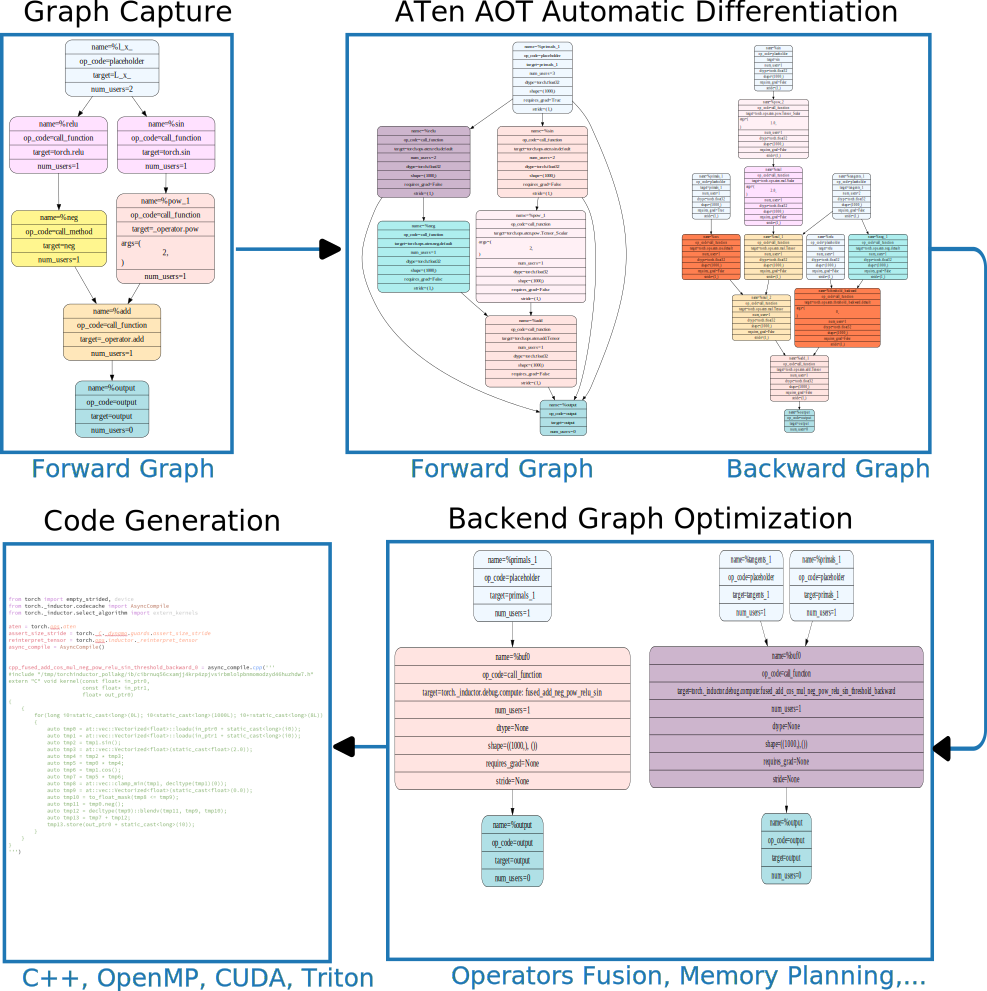
\includegraphics[width=1.0\textwidth]{pytorch_submodule/src/the_framework/graph_acquisition/figures/compile.pdf}
    \end{figure}
\end{sectionbox}
\begin{methodbox}{List Backends}
    \begin{plaincodebox}{python}
    import torch._dynamo as dynamo
    dynamo.list_backends(exclude_tags=('debug', 'experimental'))
    # 'cudagraphs', 'inductor', 'onnxrt', 'openxla', 'openxla_eval', 'tvm'
    \end{plaincodebox}
\end{methodbox}
\begin{notebox}[Backends no longer supported]\nospacing
        \begin{itemizenosep}
            \item nvFuser
        \end{itemizenosep}
\end{notebox}
%%% Local Variables:
%%% mode: latex
%%% TeX-command-extra-options: "-shell-escape"
%%% TeX-master: "../../../../../formulary"
%%% End:

    \subsubsubsection{TorchInductor}\label{subsubsec:torchinductor}
        \begin{defnbox}\nospacing
    \begin{defn}[\hfill\exampleref{example:torchinductor}\newline TorchInductor]\label{defn:torchinductor}\leavevmode\\
        TorchInductor is the default backend for \pythoninline{torch.compile} and uses:
        \begin{itemizenosep}
            \item OpenAI Triton: to produce \textit{.ptx} code for GPU hardware
            \item C++/OpenMP: for CPU targets
        \end{itemizenosep}
    \end{defn}
\end{defnbox}
%%% Local Variables:
%%% mode: latex
%%% TeX-master: "../../../../../formulary"
%%% TeX-command-extra-options: "-shell-escape"
%%% End:

    \subsubsubsection{TorchScript Compiler - maintenance mode}\label{subsubsec:torchinductor}
        \begin{defnbox}\nospacing
    \begin{defn}[Torch Script]\label{defn:torch_script}\leavevmode\\
        Troch Script uses The \textit{Neural Net Compiler} \imp{NNC} to JIT compile, optimize, fuse subgraphs.
        It then uses LLVM to generate hardware native code.
    \end{defn}
\end{defnbox}


%%% Local Variables:
%%% mode: latex
%%% TeX-command-extra-options: "-shell-escape"
%%% TeX-master: "../../../../../formulary"
%%% End:

  \subsection{OpenAI Triton}\label{subsec:openai_triton}



\section*{Building Models}\label{sec:building_models}
    \subsection{\pythoninline{torch.functional}}\label{subsec:torchinductor}
      \begin{defnbox}\nospacing
    \begin{defn}[\pythoninline{torch.functional}]\label{defn:torch_functional}\leavevmode\\
        Is a module that contains a collection of stateless functions intended for neural network operations without learnable parameters that do not change
        the way the operate between training and inference.
        But this module may also be used to build more complex custom neural network layers.
        This may include activation/loss functions, normalization, pooling layers and so on:
        \begin{mintlinebox}{python}
            import torch.nn.functional as F

            t = torch.randn(1, 1, 4, 4)
            output = F.interpolate(t, scale_factor=2, mode='bilinear')
        \end{mintlinebox}
    \end{defn}
\end{defnbox}

%%% Local Variables:
%%% mode: latex
%%% TeX-command-extra-options: "-shell-escape"
%%% TeX-master: "../../../../formulary"
%%% End:


      % parameters() Vs state_dict
      % The .parameters() only gives the module parameters i.e. weights and biases, while state_dict returns a dictionary containing a whole state of the module.
\section*{Benchmarking}\label{sec:benchmarking}
\section*{Distributed Training\hfill\normalsize{\pythoninline{import torch.distributed as dist}}}
    \begin{defnbox}\nospacing
    \begin{defn}[\hfill\tcblack{\pythoninline{torch.multiprocessing as mp}}\newline Torch Multiprocessing]\label{defn:torch_multiprocessing}
        Allows to \pythoninline{spawn} functions accros multiple processes/devices:
        \begin{mintlinebox}{python}
           ws = torch.cuda.device_count()
           mp.spawn(|\texttt{\optc{main}}|, args=(|\texttt{\optc{args\_of\_main}}|), nprocs=|\texttt{\optc{ws}}|)
        \end{mintlinebox}
        \imp{Note}: the first argument of the function must be main and gets populated automatically.
    \end{defn}
\end{defnbox}
\begin{defnbox}\nospacing
    \begin{defn}[Torch Distributed]\label{defn:torch_distributed}\leavevmode\\
        Initializes the distributed environment:
        \begin{mintlinebox}{cpp}
        def main(rank, |\texttt{\optc{ws}}|):
            os.environ("MASTER_ADDR") = |\texttt{\optc{localhost}}|
            os.environ("MASTER_PORT") = |\texttt{\optc{23456}}|
            dist.init_process_group(backend=|\texttt{\optc{backend}}|,
                                    rank=|\texttt{\optc{rank}}|,
                                    world_size=|\texttt{\optc{ws}}|)
            // Distributed Training Logic
            dist.destroy_process_group()
        \end{mintlinebox}
        \begin{itemizenosep}
            \item \pythoninline{"MASTER_ADDR"}: specifies the address (hostname or IP address) of the master node
            \item \pythoninline{"MASTER_PORT"}: specifies the port used by the backend for sending and reciveing
        \end{itemizenosep}
    \end{defn}
\end{defnbox}


%%% Local Variables:
%%% mode: latex
%%% TeX-command-extra-options: "-shell-escape"
%%% TeX-master: "../../formulary"
%%% End:

    \subsection*{Distributed Data Parallel Training}\label{subsec:distributed_data_parallel_training}
        \begin{defnbox}\nospacing
    \begin{defn}[Distributed Data Parallel\hfill\blackab{DDP}\newline \hfill\tcblack{\pythoninline{from torch.nn.parallel import DistributedDataParallel}}]\label{defn:distributeddataparallel}\leavevmode\\
        DDP wrap's our model and coordinates the training across processes/devices by synchronizing model parameters and gradient updates across the environment.
        \begin{mintlinebox}{python}
            model = DDP(model, device_ids=[|\texttt{\optc{LOCAL\_RANK}}|])|\hfill\tc{gray} model = model.module|
        \end{mintlinebox}
    \end{defn}
\end{defnbox}
\begin{notebox}[Note]\nospacing
    \texttt{\optc{LOCAL\_RANK}} is the local GPU id on which the model lives on.
\end{notebox}
\begin{attentionbox}{Attention}\nospacing
    \begin{itemizenosep}
        \item We want to save the actual module i.e. \pythoninline{model.module} to not store parameters and buffers of the DDP-wrapper model.
        \item We only want to save the model on the master rank i.e.\ \pythoninline{gpu_id==0}.
    \end{itemizenosep}
\end{attentionbox}
\begin{defnbox}\nospacing
    \begin{defn}[Distributed Sampling\newline \hfill\tcblack{\pythoninline{from torch.utils.data.distributed import DistributedSampler}}]\label{defn:distributed_sampling}\leavevmode\\
        The Distributed Sampler can be used by a \pythoninline{DataLoader} and distributes the input batch across all devices without overlap:
        \begin{mintlinebox}{python}
            dl = DataLoader(|\texttt{\optc{data}}|, batch_size=|\texttt{\optc{bs}}|, pin_memory=True,
                            shuffle=False,
                            sampler=DistributedSampler(|\texttt{\optc{data}}|))
        \end{mintlinebox}
    \end{defn}
\end{defnbox}
\begin{attentionbox}{Attention}\nospacing
    We need to set shuffle to false, as the sampler becomes responsible for distributing samples i.e.\ we don't want to pass shuffled
    samples to the sampler.
\end{attentionbox}




%%% Local Variables:
%%% mode: latex
%%% TeX-command-extra-options: "-shell-escape"
%%% TeX-master: "../../../formulary"
%%% End:

    \subsection*{Torch Run}
        \begin{defnbox}\nospacing
    \begin{defn}[Torchrun]\label{defn:torchrun}
        \pythoninline{Torchrun} is a command line script that automatically spawns processes on devices and additionally:
        \begin{itemizenosep}
            \item handles failures by restarting workers but we need to provide loading/saving logic:
            \begin{mintlinebox}{python}
            def _save_snapshot(self, epoch):
                snapshot = {
                    "MODEL_STATE": self.model.module.state_dict(),
                    "EPOCHS_RUN": epoch,
                }
                torch.save(snapshot, self.snapshot_path)
            \end{mintlinebox}
            \begin{mintlinebox}{python}
            def _load_snapshot(self, snapshot_path):
                snapshot = torch.load(snapshot_path, map_location=loc)
                self.model.load_state_dict(snapshot["MODEL_STATE"])
                self.epochs_run = snapshot["EPOCHS_RUN"]
            \end{mintlinebox}
            \item automatically sets \pythoninline{RANK} and \pythoninline{WORLD_SIZE} and \pythoninline{os.environ["LOCAL_RANK"]} to access the id of the current device.
            \item Can use an elastic number of nodes between \pythoninline{min} and \pythoninline{max}
        \end{itemizenosep}
        \imp{Simplified Initialization}:
        \begin{mintlinebox}{python}
            def main():
                dist.init_process_group(backend=|\texttt{\optc{backend}}|)
                // Distributed Training Logic
                dist.destroy_process_group()
        \end{mintlinebox}
        \imp{Execution}:
        \begingroup
        \catcode`\!=\active
        \def!#1!{\optc{\texttt{#1}}}
        \begin{mintlinebox}{bash}
           torchrun !--standalone! --nproc_per_node=gpu script.py !cmlArgs!
        \end{mintlinebox}
        \endgroup
    \end{defn}
\end{defnbox}

%%% Local Variables:
%%% mode: latex
%%% TeX-command-extra-options: "-shell-escape"
%%% TeX-master: "../../../formulary"
%%% End:


\section*{Inference}
  \section*{Torch Serve}

\newpage
\section*{Torch C++ Backend}
  \subsection*{C10}
      \begin{defnbox}\nospacing
    \begin{defn}[C10]\label{defn:c10}\leavevmode\\
        Is the core library for Pytorch
        TensorImpl, the tensor metadata structure, and the dispatcher, which is responsible for routing operator calls to the correct kernel implementation.
    \end{defn}
\end{defnbox}
\begin{notebox}[Note: name]\nospacing
   Is a play on words on \imp{c}affe2 or \imp{core} and A\imp{Ten}/\imp{Tensor}.
\end{notebox}

%%% Local Variables:
%%% mode: latex
%%% TeX-command-extra-options: "-shell-escape"
%%% TeX-master: "../../../../formulary"
%%% End:

      \subsubsection{C10 Tensor Container}\label{subsubsec:c10_tensors}
        \begin{defnbox}\nospacing
    \begin{defn}[TensorImpl\hfill\tcblack{\cppinline{c10::TensorImpl}}]\label{defn:c10::TensorImpl}\leavevmode\\
        \cppinline{c10::TensorImpl} is the PyTorch C++ Tensor container class that is associate with a single Tensor.
        It holds a reference to a \cppinline{c10::Storage} class, that represents the underlying memory storage.\\
        \cppinline{c10::TensorImpl} adds meta-data information like the data pointer, shape, strides to the \cppinline{c10::Storage}s.
    \end{defn}
\end{defnbox}
%%% Local Variables:
%%% mode: latex
%%% TeX-command-extra-options: "-shell-escape
%%% TeX-master: "../../../../../../formulary"
%%% End:

      \subsubsection{C10 Tensors}\label{subsubsec:c10_tensors}
        \begin{defnbox}\nospacing
    \begin{defn}[Tensor]\label{defn:tensor}\leavevmode\\
        Is the fundamental data structure for efficient computations in Pytorch:
        \begin{mintlinebox}{python}
            x = tensor(|\texttt{\optc{data}}|, |\texttt{\optc{[}device=\optc{device]}}|)
        \end{mintlinebox}
    \end{defn}
\end{defnbox}
\begin{corbox}\nospacing
    \begin{cor}[Implementation Details]\label{cor:torch_tensor_implementation_details}\leavevmode\\
        \pythoninline{torch.tensors} are based on the C++ ATen\cref{defn:aten} class \cppinline{at::Tensor} see \cref{defn:at::Tensor}.
    \end{cor}
\end{corbox}
%%% Local Variables:
%%% TeX-command-extra-options: "-shell-escape"
%%% mode: latex
%%% TeX-master: "../../../../../formulary"
%%% End:

  \subsection*{ATen}\label{subsec:aten}\stepcounter{subsection}
      \begin{defnbox}\nospacing
    \begin{defn}[ATen]\label{defn:aten}\leavevmode\\
        Is PyTorchs C++ Tensor Library, built on top of the C++ standard library, that defines Pytorch tensor operations.
    \end{defn}
\end{defnbox}

      \subsubsection{ATen Tensors\hfill\normalsize{\cppinline{at::Tensor}}}\label{subsubsubsec:aten_tensors}
        \begin{defnbox}\nospacing
    \begin{defn}[ATen Tensors]\label{defn:at::tensors}\leavevmode\\
        Is the basic tensor type which is an alias for \cppinline{c10::Tensor}\cref{defn:c10::Tensor}:
        \begin{mintlinebox}{C++}
            #include <ATen/ATen.h>
            at::Tensor a = |\texttt{\optc{create\_or\_assign\_tensor()}}|;
        \end{mintlinebox}
    \end{defn}
\end{defnbox}

%%% Local Variables:
%%% mode: latex
%%% TeX-command-extra-options: "-shell-escape"
%%% TeX-master: "../../../../formulary"
%%% End:

      \subsubsection*{Autograd}\label{subsec:autograd}\stepcounter{subsection}
      \subsubsection*{C++ Frontend}\label{subsec:c++_frontend}\stepcounter{subsection}
      \subsubsection*{TorchScript}\label{subsec:torchscript}\stepcounter{subsection}
      \subsubsection*{C++ Extension}\label{subsec:c++_extension}\stepcounter{subsection}

  \subsection*{torch/csrc}
      \begin{defnbox}\nospacing
    \begin{defn}[torch/csrc]\label{defn:torchcsrc}\leavevmode\\
        Contains the C++ source code for torch and relies heavily on C10 and ATen.
    \end{defn}
\end{defnbox}

%%% Local Variables:
%%% mode: latex
%%% TeX-command-extra-options: "-shell-escape"
%%% TeX-master: "../../../../../formulary"
%%% End:

      \subsubsection{Autograd}\label{subsubsec:autograd}
        \begin{defnbox}\nospacing
    \begin{defn}[\hfill\tcblack{\texttt{torch/csrc/autograd/variable.h}}\newline
        AutogradMeta]\label{defn:autogradmeta}\leavevmode\\
        Is a data structure that hold graph information required for automatic differentiation:
        \begin{mintlinebox}{cpp}
            struct TORCH_API AutogradMeta : public c10::AutogradMetaInterface {
                std::string name_;

                Variable grad_;
                std::shared_ptr<Node> grad_fn_;
                std::weak_ptr<Node> grad_accumulator_;
                // other fields and methods
                ...
            };
        \end{mintlinebox}
    \end{defn}
\end{defnbox}
\begin{notebox}[Note]\nospacing
    \begin{itemizenosep}
        \item Each tensor that requires a gradient obtains a reference to such a structure.
        \item \texttt{TORCH\_API} is a macro that sets the visibility of the function of the shared library i.e.
        for GCC \cppinline{__attribute__((__visibility__("default")))}.
        By default functions are not exposed in the shared library.
    \end{itemizenosep}
\end{notebox}

%%% Local Variables:
%%% mode: latex
%%% TeX-command-extra-options: "-shell-escape"
%%% TeX-master: "../../../../../formulary"
%%% End:







\newpage
\section{Examples}
  \subsection{Pytorch Internals}\label{subsec:pytorch_internals}
  \begin{examplebox}\nospacing
    \begin{example}[TorchInductor\cref{defn:torchinductor}]\label{example:torchinductor}\leavevmode\\
        Using the options \pythoninline{trace.enabled} and \pythoninline{trace.graph_diagram} will create the folders:
        \begin{itemize}
            \item \texttt{torch\_compile\_debug/run\_\optc{<DATE\_TIME\_PID>}/aot\_torchinductor/}
            \item \texttt{model\_\_\optc{XX}\_\optc{(forward/backward)}\_\optc{XX}/output\_code.py}
        \end{itemize}
        that include the forward and backward code:
        \begin{plaincodebox}{python}
        import torch
        import torch._dynamo as dynamo
        from functorch.compile import make_boxed_func
        from torch.fx.passes.graph_drawer import FxGraphDrawer

        def fu(x: torch.Tensor):
            return torch.relu(x).neg() + torch.sin(x) ** 2

        dynamo.reset()
        cmp_f = torch.compile(fu,
            backend="inductor",
            options={"trace.enabled": True, "trace.graph_diagram": True}
        )
        device = "cpu" # device = 'gpu'
        x = torch.rand(1000, requires_grad=True).to(device)
        y = torch.ones_like(x)
        out = torch.nn.functional.mse_loss(cmp_f(x), y).backward()
        \end{plaincodebox}
    \end{example}
\end{examplebox}

  \begin{examplebox}\nospacing
    \begin{example}[TorchInductor\cref{defn:torchinductor}]\label{example:torchinductor}\leavevmode\\
        Using the options \pythoninline{trace.enabled} and \pythoninline{trace.graph_diagram} will create the folders:
        \begin{itemize}
            \item \texttt{torch\_compile\_debug/run\_\optc{<DATE\_TIME\_PID>}/aot\_torchinductor/}
            \item \texttt{model\_\_\optc{XX}\_\optc{(forward/backward)}\_\optc{XX}/output\_code.py}
        \end{itemize}
        that include the forward and backward code:
        \begin{plaincodebox}{python}
        import torch
        import torch._dynamo as dynamo
        from functorch.compile import make_boxed_func
        from torch.fx.passes.graph_drawer import FxGraphDrawer

        def fu(x: torch.Tensor):
            return torch.relu(x).neg() + torch.sin(x) ** 2

        dynamo.reset()
        cmp_f = torch.compile(fu,
            backend="inductor",
            options={"trace.enabled": True, "trace.graph_diagram": True}
        )
        device = "cpu" # device = 'gpu'
        x = torch.rand(1000, requires_grad=True).to(device)
        y = torch.ones_like(x)
        out = torch.nn.functional.mse_loss(cmp_f(x), y).backward()
        \end{plaincodebox}
    \end{example}
\end{examplebox}

  \begin{examplebox}\nospacing
    \begin{example}[TorchInductor\cref{defn:torchinductor}]\label{example:torchinductor}\leavevmode\\
        Using the options \pythoninline{trace.enabled} and \pythoninline{trace.graph_diagram} will create the folders:
        \begin{itemize}
            \item \texttt{torch\_compile\_debug/run\_\optc{<DATE\_TIME\_PID>}/aot\_torchinductor/}
            \item \texttt{model\_\_\optc{XX}\_\optc{(forward/backward)}\_\optc{XX}/output\_code.py}
        \end{itemize}
        that include the forward and backward code:
        \begin{plaincodebox}{python}
        import torch
        import torch._dynamo as dynamo
        from functorch.compile import make_boxed_func
        from torch.fx.passes.graph_drawer import FxGraphDrawer

        def fu(x: torch.Tensor):
            return torch.relu(x).neg() + torch.sin(x) ** 2

        dynamo.reset()
        cmp_f = torch.compile(fu,
            backend="inductor",
            options={"trace.enabled": True, "trace.graph_diagram": True}
        )
        device = "cpu" # device = 'gpu'
        x = torch.rand(1000, requires_grad=True).to(device)
        y = torch.ones_like(x)
        out = torch.nn.functional.mse_loss(cmp_f(x), y).backward()
        \end{plaincodebox}
    \end{example}
\end{examplebox}

  \subsubsection{Dynamic Graphs}\label{subsubsec:dynamic_graphs}
    \begin{examplebox}\nospacing
    \begin{example}[Data Dependent Control Flow]\label{example:data_dependent_control_flow}\leavevmode
        \begin{plaincodebox}{python}
            def fu(x):
                if x.sum() < 0:
                    return torch.tensor(0)
                return torch.tensor(1)
            x = torch.randn(5, 5)
            jit_fu = jit.trace(fu, (x,))
            fx_fu = fx.symbolic_trace.trace(fu, concrete_args={'x': x})
            dynamo_fu = dynamo.optimize(fu, (x,))
            jit_fu(-x) # != fu(x)
            fx_fu(-x) # != fu(x)
            dynamo_fu(-x) # == fu(x)
        \end{plaincodebox}
    \end{example}
\end{examplebox}
\begin{examplebox}\nospacing
    \begin{example}[Module Dependent Control Flow]\label{example:module_dependent_control_flow}\leavevmode\\
        After jit compilation\pythoninline{x = scipy.fft.dct(x.numpy())} and \pythoninline{x = torch.from_numpy(x)} will be treated as constants by \pythoninline{torch.fx} and \pythoninline{torch.jit}:
        \begin{plaincodebox}{python}
        def fu(x):
            x = x*2
            x = scipy.fft.dct(x.numpy())
            x = torch.from_numpy(x)
            x = x * 2
            return x
        x = torch.randn(5, 5)
        jit_fu = jit.trace(fu, (x,))
        fx_fu = fx.symbolic_trace.trace(fu, concrete_args={'x': x})
        dynamo_fu = dynamo.optimize(fu, (x,))
        jit_fu(-x) # != fu(x)
        fx_fu(-x) # != fu(x)
        dynamo_fu(-x) # == fu(x)
        \end{plaincodebox}
    \end{example}
\end{examplebox}

  \subsubsection{Troch Inductor}\label{subsubsec:dynamic_graphs}
    \begin{examplebox}\nospacing
    \begin{example}[TorchInductor\cref{defn:torchinductor}]\label{example:torchinductor}\leavevmode\\
        Using the options \pythoninline{trace.enabled} and \pythoninline{trace.graph_diagram} will create the folders:
        \begin{itemize}
            \item \texttt{torch\_compile\_debug/run\_\optc{<DATE\_TIME\_PID>}/aot\_torchinductor/}
            \item \texttt{model\_\_\optc{XX}\_\optc{(forward/backward)}\_\optc{XX}/output\_code.py}
        \end{itemize}
        that include the forward and backward code:
        \begin{plaincodebox}{python}
        import torch
        import torch._dynamo as dynamo
        from functorch.compile import make_boxed_func
        from torch.fx.passes.graph_drawer import FxGraphDrawer

        def fu(x: torch.Tensor):
            return torch.relu(x).neg() + torch.sin(x) ** 2

        dynamo.reset()
        cmp_f = torch.compile(fu,
            backend="inductor",
            options={"trace.enabled": True, "trace.graph_diagram": True}
        )
        device = "cpu" # device = 'gpu'
        x = torch.rand(1000, requires_grad=True).to(device)
        y = torch.ones_like(x)
        out = torch.nn.functional.mse_loss(cmp_f(x), y).backward()
        \end{plaincodebox}
    \end{example}
\end{examplebox}






%%% Local Variables:
%%% mode: latex
%%% TeX-command-extra-options: "-shell-escape"
%%% TeX-master: "../formulary"
%%% End:
